\subsection{Chebyshev polynomials and series}
Again, instead of using trigonometric polynomials, try to apply another system of orthogonal polynomials - Chebyshev polynomials and expansion into the Chebyshev series. 
The Chebyshev polynomials can be defined as the recurrent sequence:
\begin{equation}
	T_0(x) = 1, T_1(x) = x, \dots, T_n(x) = 2 x T_{n - 1}(x) - T_{n - 2}(x)
\end{equation}
This polynomials are orthogonal with weight $w(x) = \dfrac{1}{\sqrt{1 - x^2}}$\cite{mason2002chebyshev}:
\begin{equation}
	\label{eq:chebyshev_series}
	\int_{-1}^{1} T_k(x) T_l(x) w(x) dx = \begin{cases}
		\pi \delta_l^k, k = 0, \\
		\cfrac{1}{2} \pi \delta_l^k, k \neq 0
	\end{cases}
\end{equation}
Examples of the first six polynomials are plotted at the \ref{fig:chebyshev_demo}
\begin{figure}[h]
	\centering
	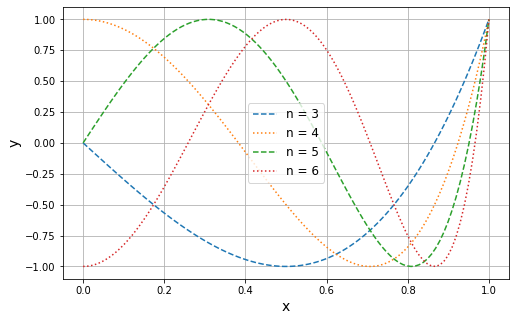
\includegraphics[width=0.65 \textwidth]{images/chapter2/chebyshev_demo.png}
	\caption{Chebyshev polynomias for n = 3, 4, 5, 6}
	\label{fig:chebyshev_demo}
\end{figure}

These polynomials are used for the interpolation procedure to avoid the Runge phenomenon\footnote{In the mathematical field of numerical analysis, Runge's phenomenon is a problem of oscillation at the edges of an interval that occurs when using polynomial interpolation with polynomials of high degree over a set of equispaced interpolation points.}, in case, when they are monic polynomials. Moreover, the roots of them often used in numerical linear algebra in method conjugated gradient descent, for example\footnote{
More information is here - ``E. Kaporin, Using Chebyshev polynomials and approximate inverse triangular
factorizations for preconditioning the conjugate gradient method, Zh. Vychisl. Mat.
Mat. Fiz., 2012, Volume 52, Number 2, 179–204``}.
The details of the Chebyshev polynomials is not important for this work, but there are a lot of benefit of using them in different problems.

Chebyshev series is the expansion of the function by his polynomials or, simply substitute polynomials to \eqref{eq:linear_expansion}:
\begin{equation*}
	\begin{multlined}
		f(x) = \sum_{k = 0}^{\infty} c_k T_k(x) \\
		c_k = \dfrac{1}{M} \int_{-1}^1 f(x) T_k(x) w(x) dx, \text{where } M = \begin{cases}
		\pi, k = 0, \\
		\dfrac{1}{2} \pi, k \neq 0
	\end{cases} \\
	\text{and } w(x) \text{ weight function } = \dfrac{1}{\sqrt{1 - x^2}}
	\end{multlined}
\end{equation*}

And the convergence theorem.
\begin{theorem}
\label{chevyshev_convergence}
When a function $f$ has $m + 1$ continous derivatives on $[-1, 1]$ or $ f \in C^{m + 1}[-1, 1] $, where $m \in N^+$, then $\| f(x) - S_k(x) \| = \mathcal{O}\left ( \dfrac{1}{k^m} \right )$ as $k \rightarrow \infty \quad \forall x \in [-1, 1]$ 
\end{theorem}
The proof here \cite{mason2002chebyshev}.
This theorem described the same fact that theorem \ref{convergence-l2-norm}  described for the Fourier expansion.

\paragraph{Example of Chebyshev interpolation}
Consider the function $y = sin(x) + x cos(x)$ and at the fig. \ref{fig:chebyshev_expansion} the results. 
\begin{figure}[h]
	\centering
	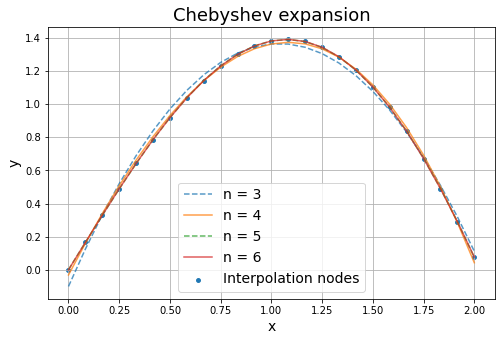
\includegraphics[width=0.7 \textwidth]{images/chapter2/chebyshev_series.png}
	\caption{Chebyshev expansion with 3, 4, 5, 6 terms }
	\label{fig:chebyshev_expansion}
\end{figure}


In fact, Chebyshev series is Generalized Fourier series: 
\begin{equation*}
	\begin{multlined}
		f(x) = \sum_{i = 1}^{N} c_n \phi_n(x) \\
		\left < \phi_i, \phi_j \right > = \int_{V} \phi_i \phi_j w dV = K \delta_i^j
	\end{multlined}
\end{equation*}
